The purpose of this section is to answer both the checkpoint and report
questions of the lab, as well as discuss any relevant results obtained during the experiences.

\subsection{Part 1: Wheatstone Bridge}

\begin{enumerate}

\item \textbf{Place a voltmeter to measure the potential difference between nodes A and B.}

The potencial difference between nodes A and B was $46.0656\,\mathrm{pV}$.

\begin{figure}[htbp]
    \centering
    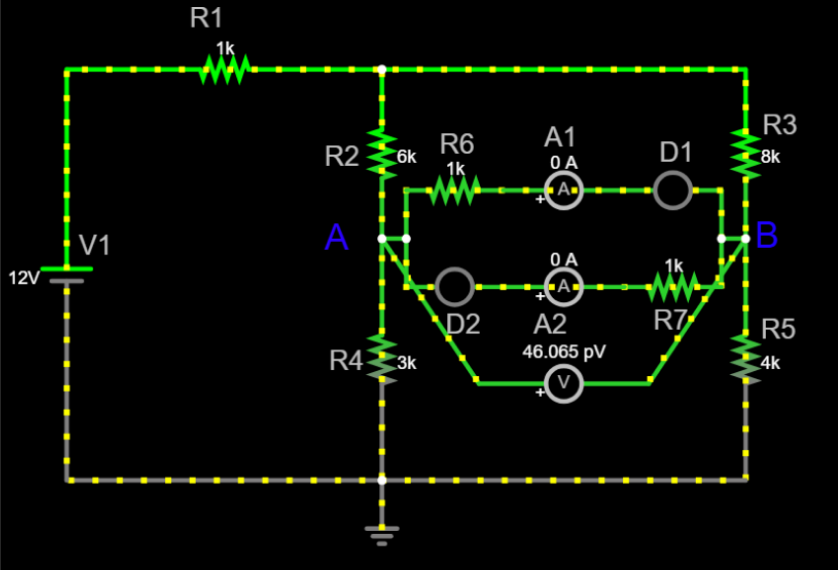
\includegraphics[width=1\linewidth]{img/1.png}
    \caption{Initial Wheatstone bridge circuit implemented in Falstad with the voltmeter and ammeter.}\label{fig:1}
\end{figure}

\item \textbf{Using the measurement tools:}

\begin{enumerate}
    \item \textbf{Measure the currents and voltages across resistors R2, R3, R4, and R5.}
    \par \vspace{0.15cm}
    The measured current and voltage values were as follows:
    \begin{itemize}
        \item R2: $I_{R2}=1.116\,\mathrm{mA}$ and $V_{R2}=6.698\,\mathrm{V}$.
        \item R3: $I_{R3}=837.209\,\mathrm{\mu A}$ and $V_{R3}=6.698\,\mathrm{V}$.
        \item R4: $I_{R4}=1.116\,\mathrm{mA}$ and $V_{R4}=3.349\,\mathrm{V}$.
        \item R5: $I_{R5}=837.209\,\mathrm{\mu A}$ and $V_{R5}=3.349\,\mathrm{V}$.
    \end{itemize}
    \item \textbf{Measure the current flowing through diodes D1 and D2.}
    \par \vspace{0.15cm}
    The current through both diodes was approximately zero:
    \[
        I_{D1}=0\,\mathrm{A},
        \qquad
        I_{D2}=0\,\mathrm{A}.
    \]
    \item \textbf{Change the resistance of R5 to $8\,\mathrm{k\Omega}$. What changes are observed in the ammeters and the voltmeter located in the central branch?}
    \par \vspace{0.15cm}
    Before changing R5, the central-branch voltmeter measured approximately $46.066\,\mathrm{pV}$,
    while both ammeters measured $0\,\mathrm{A}$. After changing R5 to $8\,\mathrm{k\Omega}$, the
    voltmeter measured $-1.348\,\mathrm{V}$, while the ammeters measured $-93.2\,\mathrm{pA}$ and
    $-59.02\,\mathrm{\mu A}$, respectively. These results indicate that changing R5 unbalanced the
    bridge and produced current flow through the central branch.
    \begin{figure}[htbp]
        \centering
        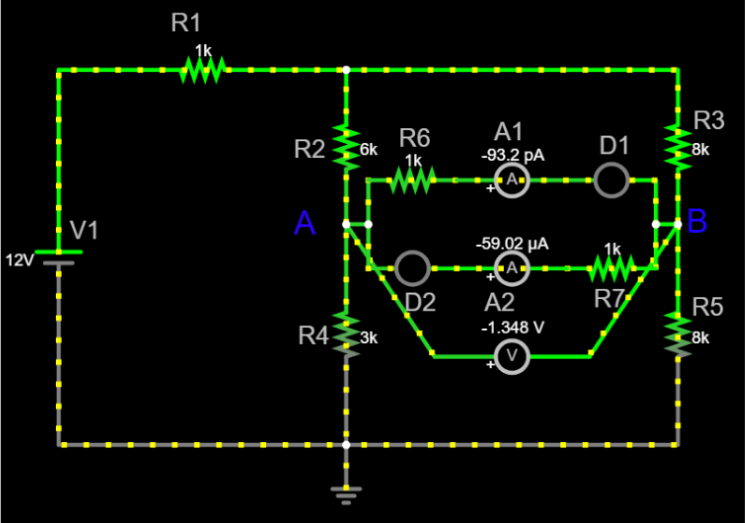
\includegraphics[width=1\linewidth]{img/2.png}
        \caption{Wheatstone bridge measurements after changing resistor R5}\label{fig:2}
    \end{figure}
    
\end{enumerate}

\item \textbf{Reverse the polarity of the voltage source. Are the currents through the diodes affected?}
\par \vspace{0.15cm}
Reversing the polarity of the voltage source affected the currents through the diodes. The measured currents were $I_{D1}=59.02\,\mathrm{\mu A}$ and $I_{D2}=-93.2\,\mathrm{pA}$. Therefore, D1 was forward-biased and conducted current, whereas the current through D2 was practically zero, indicating that D2 was reverse-biased.

\begin{figure}[htbp]
    \centering
    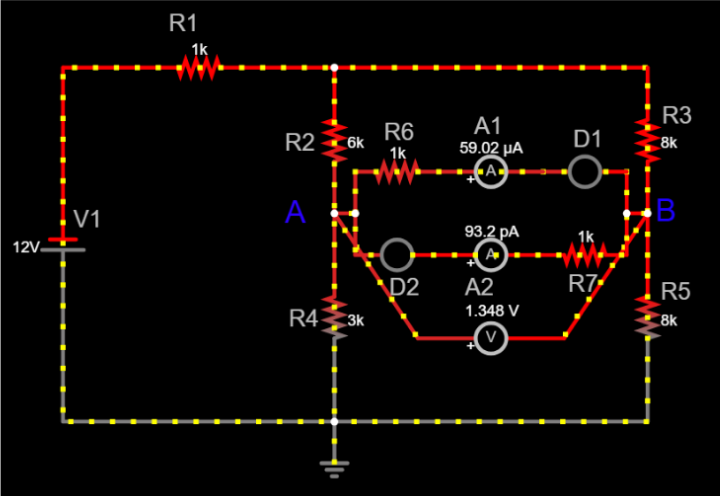
\includegraphics[width=1\linewidth]{img/3.png}
    \caption{Wheatstone bridge simulation after reversing the polarity of the voltage source.}\label{fig:3}
\end{figure}

\end{enumerate}




\subsection{Part 1: Simulation exercise in Tinkercad}

Using the measurement tools, do the following:
\begin{enumerate}
    \item \textbf{Determine the value of the current supplied by the voltage source.}
    \par \vspace{0.15cm}
    The current supplied by the voltage source was $1.13\,\mathrm{mA}$.
    \begin{figure}[htbp]
        \centering
        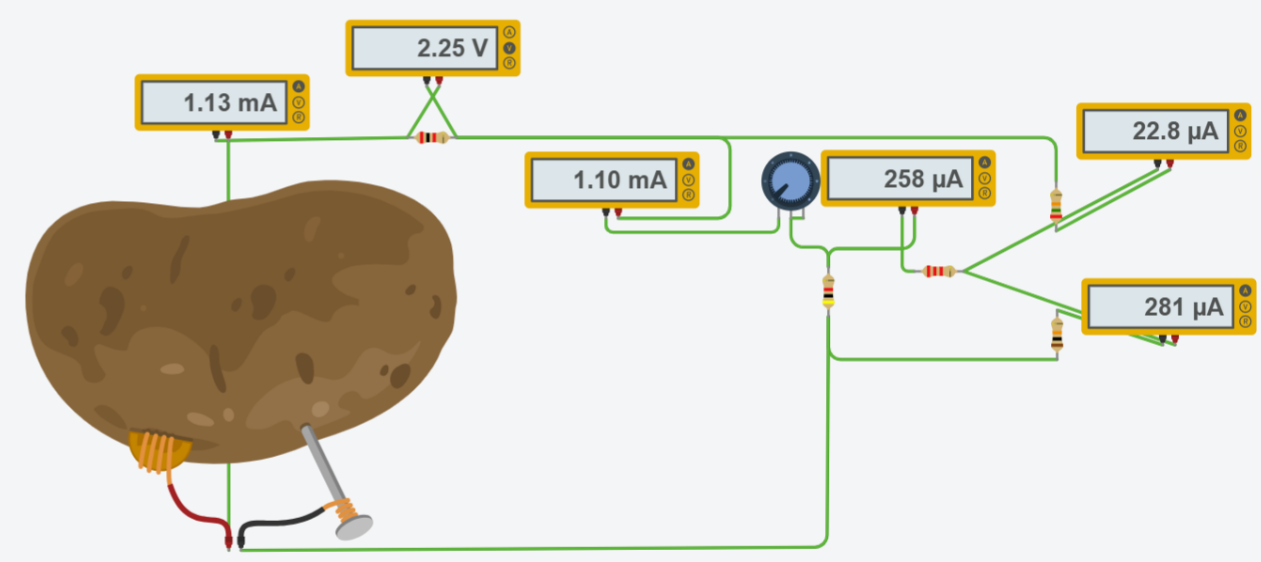
\includegraphics[width=1\linewidth]{img/4.png}
        \caption{Measurement of the total current supplied by the voltage source in the Tinkercad Wheatstone bridge simulation.}\label{fig:4}
    \end{figure}
    
    \item \textbf{Turn the potentiometer knob to its minimum value. What is the current flowing through the potentiometer?}
    \par \vspace{0.15cm}
    When the potentiometer was set to its minimum value, the current was $1.10\,\mathrm{mA}$.
    \begin{figure}[htbp]
        \centering
        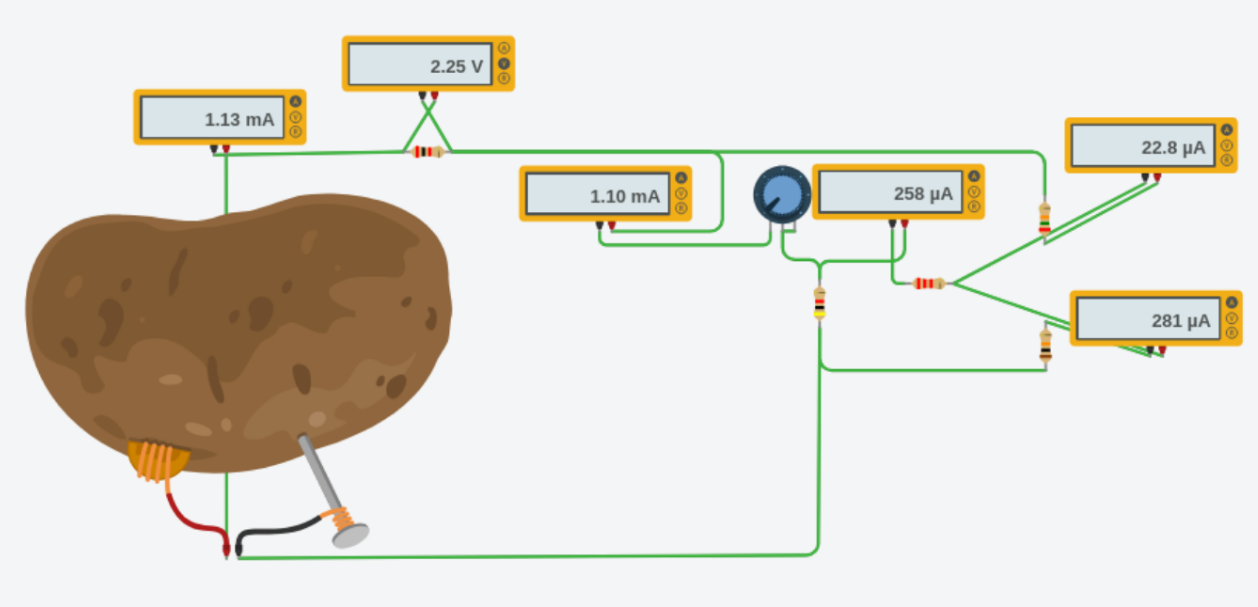
\includegraphics[width=1\linewidth]{img/5.png}
        \caption{Current measurement with the potentiometer set to its minimum resistance.}\label{fig:5}
    \end{figure}
    
    \item \textbf{Turn the potentiometer knob to its maximum value. What is the current flowing through the potentiometer now?}
    \par \vspace{0.15cm}
    When the potentiometer was set to its maximum value, the measured current through the potentiometer was $486\,\mathrm{\mu A}$.
    \begin{figure}[htbp]
        \centering
        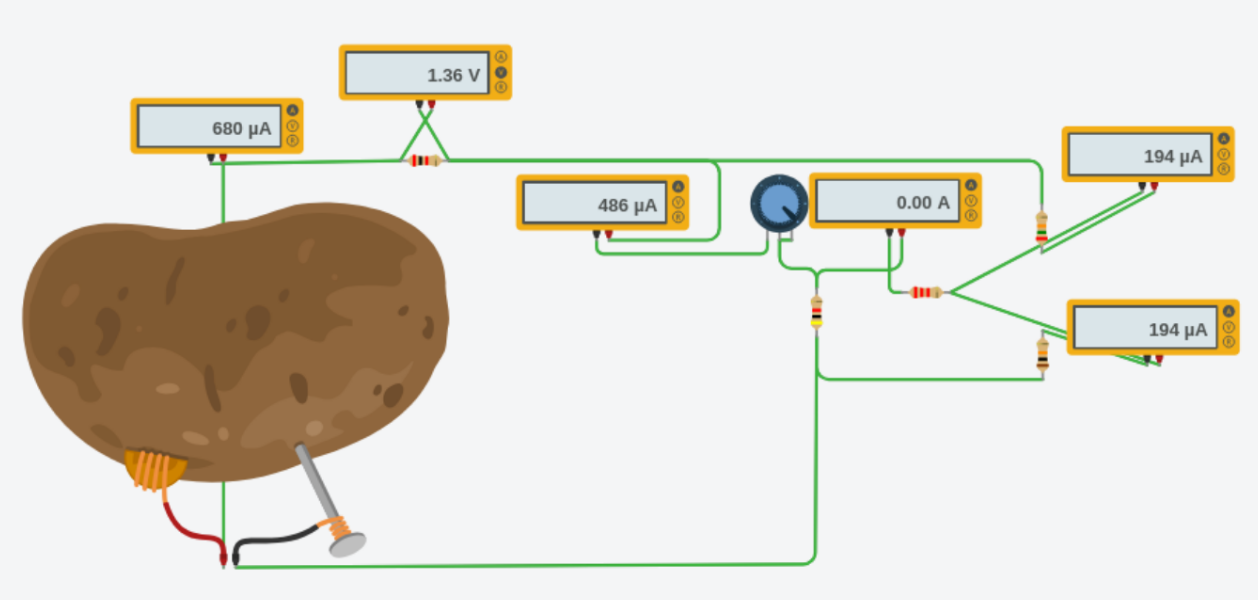
\includegraphics[width=1\linewidth]{img/6.png}
        \caption{Voltage and current measurements under the balanced condition of the Wheatstone bridge.}\label{fig:6}
    \end{figure}
    
    \item \textbf{What is the resistance of the potentiometer under the balanced condition?}      
    \par \vspace{0.15cm}
    Under the balanced condition, the potentiometer resistance was $10\,\mathrm{k\Omega}$.
    
    \item \textbf{Measure the voltage drop across resistor R0.}     
    \par \vspace{0.15cm}
    The measured voltage drop across R0 was $1.36\,\mathrm{V}$.
    
    \item \textbf{Under this condition, what are the currents and voltages across resistors R2 and R4? Are any of these values equal? Explain why.}      
    \par \vspace{0.15cm}
    The voltage drops across R2 and R4 were $4.86\,\mathrm{V}$ and $1.94\,\mathrm{V}$, respectively. Both resistors carried the same current of $194\,\mathrm{\mu A}$. Since the bridge was balanced, no current flowed through the central branch. Consequently, R2 and R4 behaved as components connected
    in series and carried the same current.
\end{enumerate}

\subsection{Part 1: LED Diode}
Do the following:
\begin{enumerate}
    \item \textbf{Measure the forward-bias voltage of each diode using the measurement tools. Include a screenshot showing all the measured values.}
    \begin{itemize}
        \item Red LED $= 2.02\,\mathrm{V}$
        \item Blue LED $= 3.68\,\mathrm{V}$
        \item Green LED $= 2.43\,\mathrm{V}$
        \item White LED: $= 3.34\,\mathrm{V}$
        \item Silicon diode: $= 612\,\mathrm{mV}$
    \end{itemize}
    \begin{figure}[htbp]
        \centering
        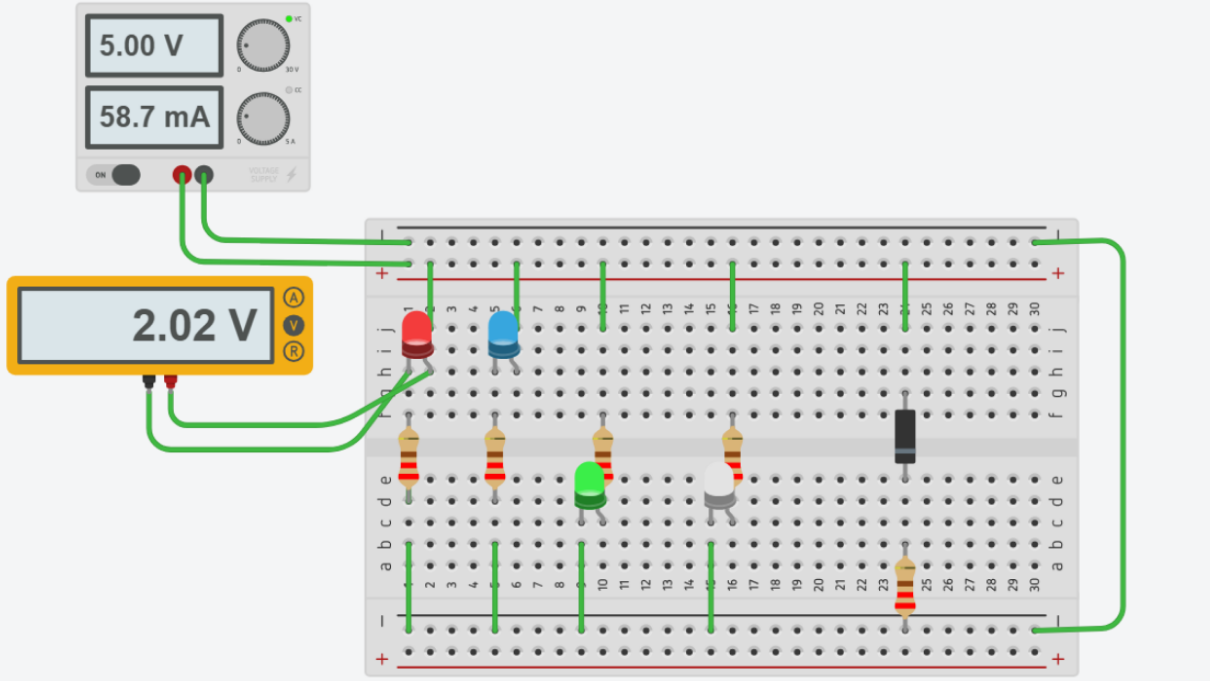
\includegraphics[width=1\linewidth]{img/7.png}
        \caption{Voltage measured across the red LED.}\label{fig:7}
    \end{figure}
    \begin{figure}[htbp]
        \centering
        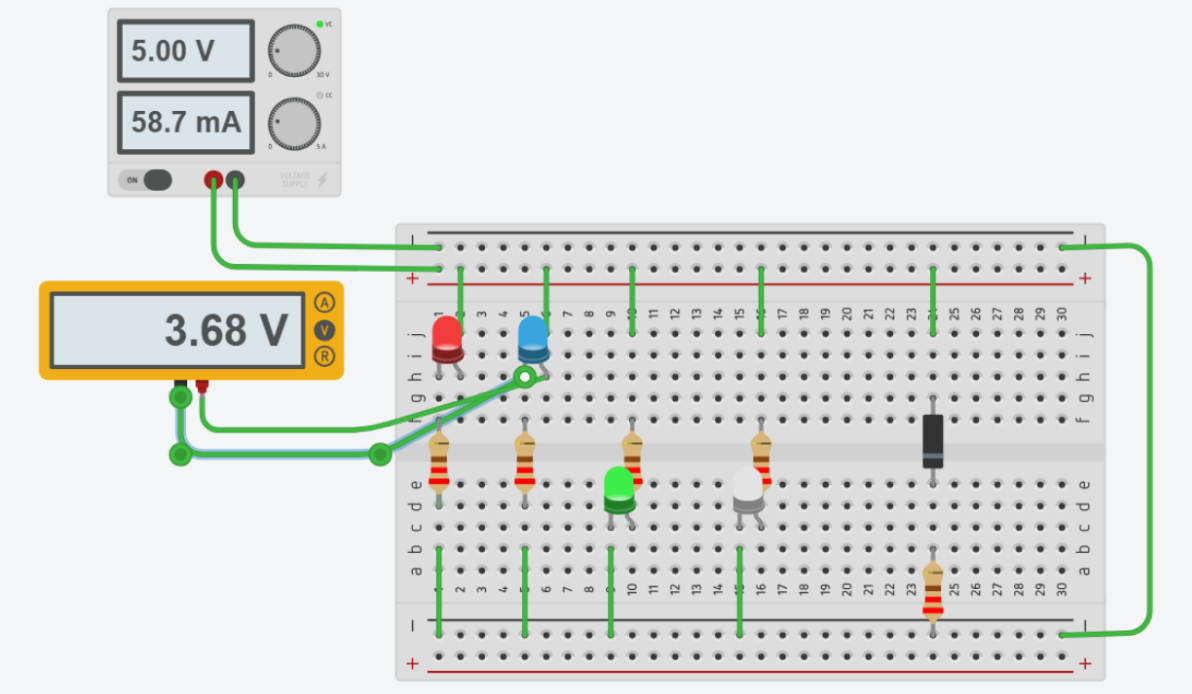
\includegraphics[width=1\linewidth]{img/8.png}
        \caption{Voltage measured across the blue LED.}\label{fig:8}
    \end{figure}
    \begin{figure}[htbp]
        \centering
        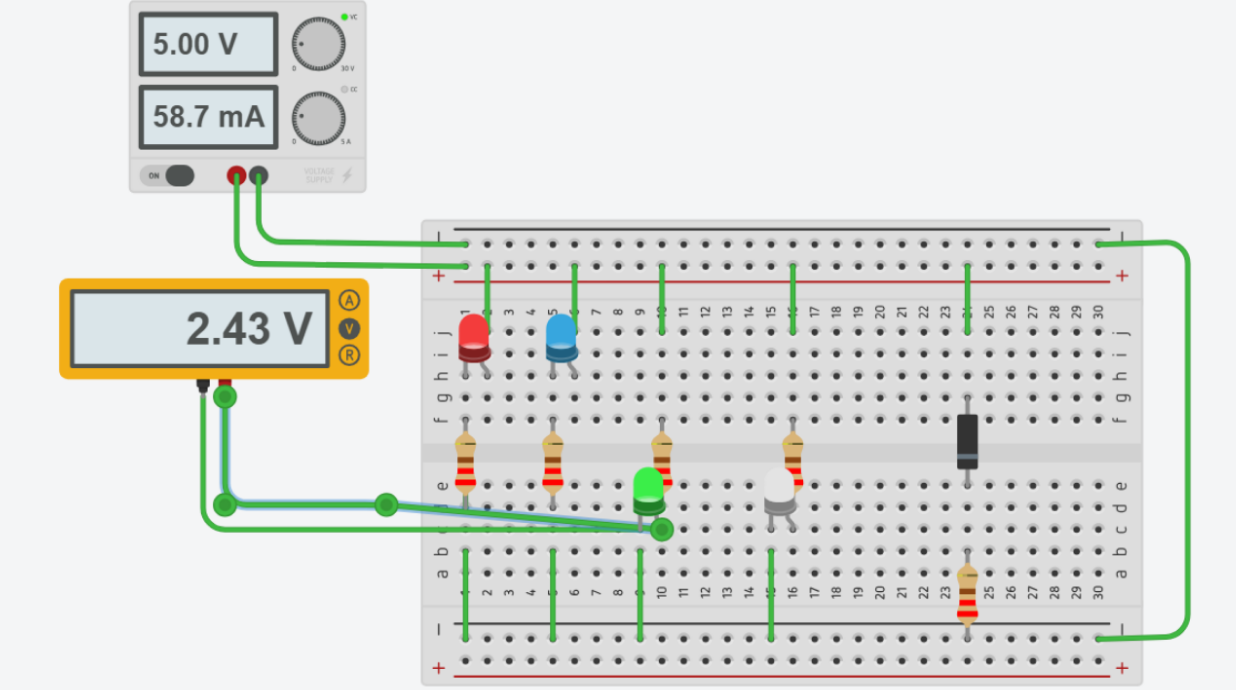
\includegraphics[width=1\linewidth]{img/9.png}
        \caption{Voltage measured across the green LED.}\label{fig:9}
    \end{figure}
    \begin{figure}[htbp]
        \centering
        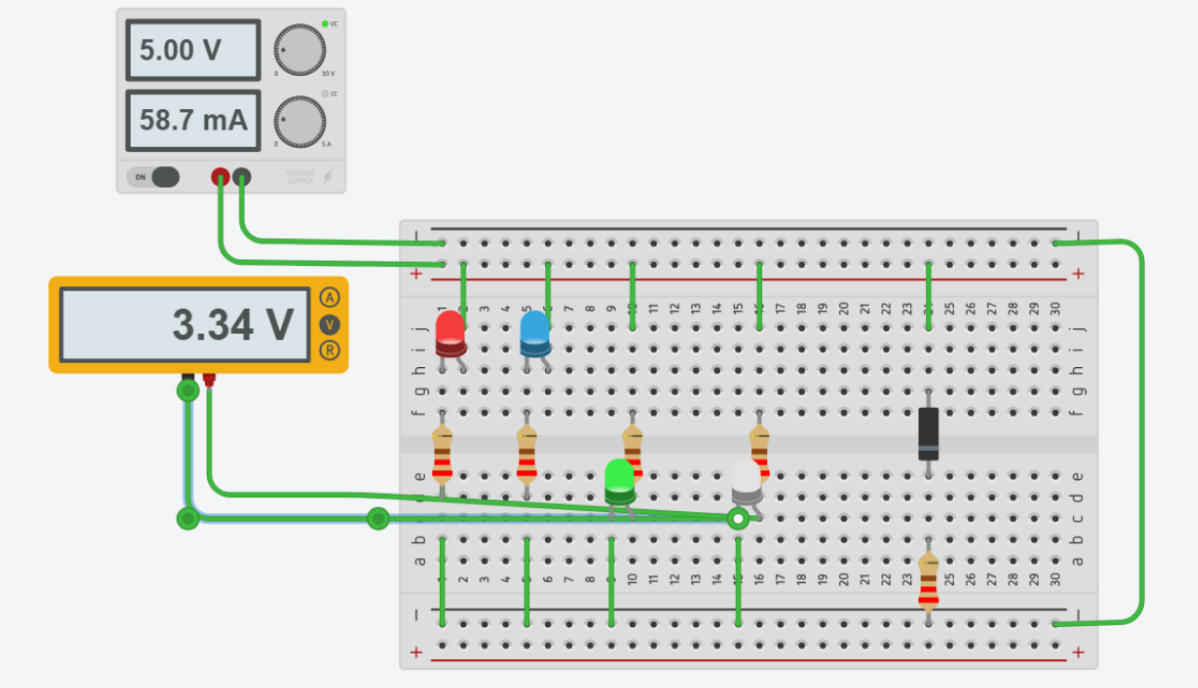
\includegraphics[width=1\linewidth]{img/10.png}
        \caption{Voltage measured across the white LED.}\label{fig:10}
    \end{figure}
    \begin{figure}[htbp]
        \centering
        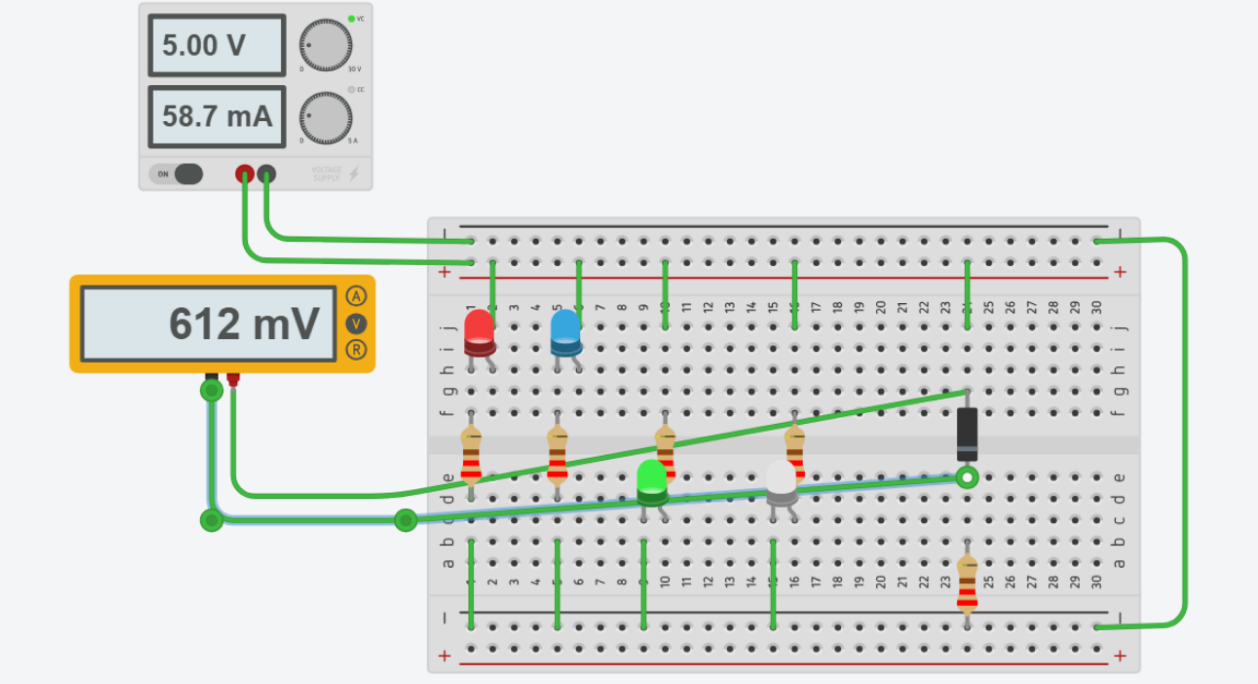
\includegraphics[width=1\linewidth]{img/11.png}
        \caption{Voltage measured across the silicone diode.}\label{fig:11}
    \end{figure}
    
    \item \textbf{Compare the forward voltage of an LED with that of a silicon diode. What difference is observed?}     
    \par \vspace{0.15cm}
    The LEDs exhibited a higher voltage than the conventional silicon diode. In this circuit, the silicon diode voltage was approximately $21.34\%$ of the highest LED forward voltage.

    \item \textbf{Which LED color has the highest forward-bias voltage?}     
    \par \vspace{0.15cm}
    The blue LED had the highest forward-bias voltage, with a measured value of $3.68\,\mathrm{V}$.

    \item \textbf{Change all resistor values to $1\,\mathrm{k\Omega}$. Do all the LEDs operate normally?}     
    \par \vspace{0.15cm}
    After changing all the resistors to $1\,\mathrm{k\Omega}$, the current through each branch decreased. Consequently, the LEDs did not emit light with the same intensity.
    \begin{figure}[htbp]
        \centering
        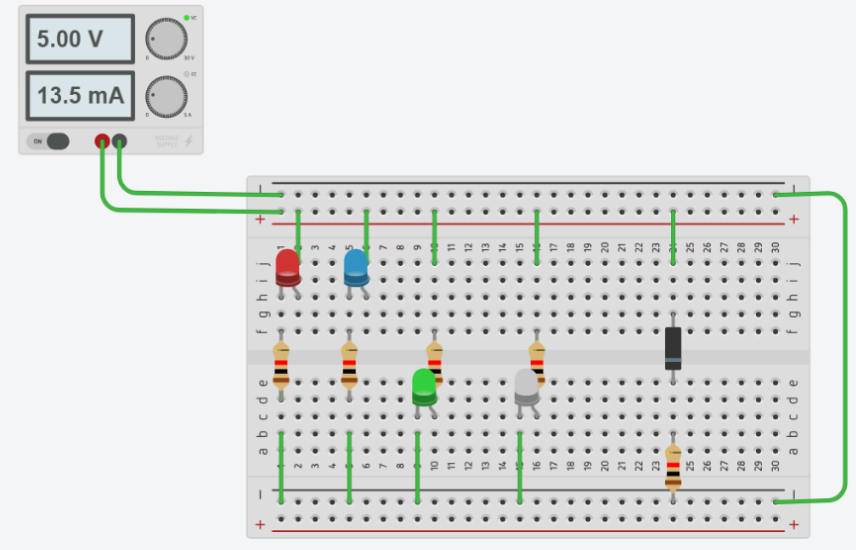
\includegraphics[width=1\linewidth]{img/12.png}
        \caption{LED circuit simulation after changing all current-limiting resistors to $1\,\mathrm{k\Omega}$.}\label{fig:12}
    \end{figure}
    
    \item \textbf{Replace the voltage source with a $3.3\,\mathrm{V}$ battery. Do all the LEDs operate normally?}      
    \par \vspace{0.15cm}
    After replacing the power supply with a $3.3\,\mathrm{V}$ source, not all the LEDs operated normally. LEDs whose 
    voltage requirements were close to or greater than the available voltage emitted very little light or did not turn on.
    \begin{figure}[htbp]
        \centering
        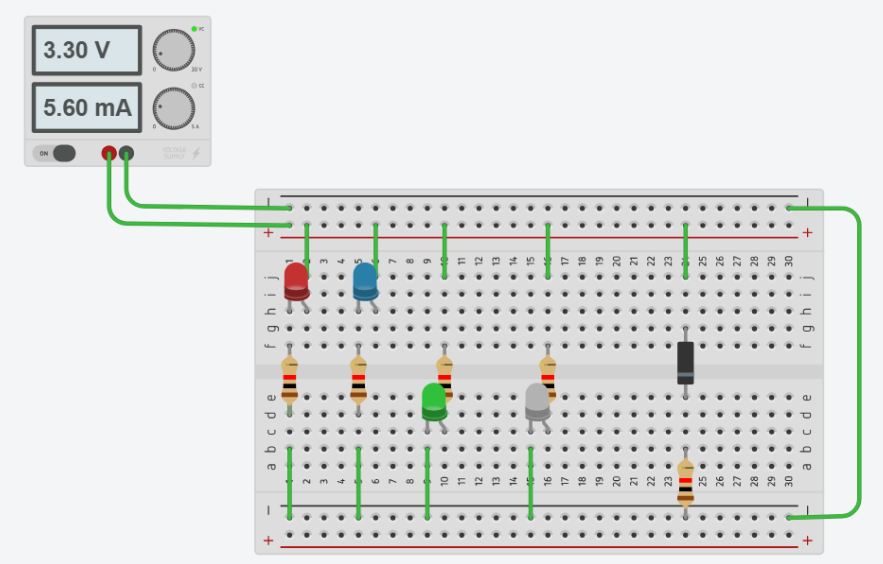
\includegraphics[width=1\linewidth]{img/13.png}
        \caption{LED circuit simulation after changing voltage source to $3.3\,\mathrm{V}$ battery.}\label{fig:13}
    \end{figure}
\end{enumerate}


\subsection{Part 2: Breadboard implementation}
\begin{enumerate}
    \item Assemble the circuit shown in the laboratory guide on the breadboard, following the specified configuration for each branch.
    \par \vspace{0.15cm}
    The operation of the circuit is demonstrated in the following video: \href{https://drive.google.com/file/d/1wEC5qJdxwSSljLp7xxYoH1fwVQjpyCVe/view?usp=sharing}{\textbf{Video evidence of the breadboard implementation}}.
    \item \textbf{Branches 1 and 2:} Qualitatively compare the brightness of red LED 1 and red LED 2.
    \par \vspace{0.15cm}
    In Branches 1 and 2, red LED 1 appeared brighter than red LED 2. This difference was caused by the different current-limiting resistances used in the two branches. A lower series resistance allowed a greater current to flow through the LED, producing greater brightness.

    \item \textbf{Branch 3:} What happens to the brightness of the LEDs? Why does this occur?
    \par \vspace{0.15cm}
    In Branch 3, the brightness of the LEDs decreased. Because the LEDs were connected in series, the supply voltage was divided among them. The available voltage and current were therefore insufficient for both LEDs to operate at their normal brightness.

    \item \textbf{Branch 4:} Set the potentiometer to its midpoint and connect the blue LED. Adjust the knob to obtain the minimum and maximum brightness. In both cases, measure the voltage across the potentiometer using the multimeter as a voltmeter.
    \par \vspace{0.15cm}
    In Branch 4, adjusting the potentiometer changed its effective resistance and consequently controlled the current flowing through the blue LED. Increasing the resistance reduced the current and produced minimum brightness, whereas decreasing the resistance increased the current and produced maximum brightness. The corresponding potentiometer voltages were measured for both conditions.

    
    \item \textbf{Branch 5:} What happens to the diodes? Why? 
    \par \vspace{0.15cm}
    In Branch 5, neither LED turned on because the two diodes were connected in opposite directions in series. For either polarity of the supply voltage, one diode was forward-biased while the other was reverse-biased. The reverse-biased diode blocked the current through the entire branch.
\end{enumerate}

\subsection{Part 2: Timing Control and Asynchronous Events}
\begin{itemize}
    \item The physical operation of the system is demonstrated in the following video: \href{https://drive.google.com/file/d/1NkIKRR5Uljy8n8Y9riXQXsNsNZCVbqpO/view?usp=drive_link}{view video demonstration}.
    
    \item The corresponding Tinkercad simulation is available at: \href{https://www.tinkercad.com/things/3kCfc5MDe2a/editel?returnTo=%2Fdashboard%2Fdesigns%2Fcircuits&sharecode=oP2IA3rm0lyTK2qXPQhzvKKvkRX0EfQxZIho4yMRpsc}{view Tinkercad simulation}.
\end{itemize}


\subsection{Part 2: Matrix Keypad Access System and Serial Feedback}
\begin{itemize}
    \item The physical operation of the matrix keypad access system is demonstrated in the following video: \href{https://drive.google.com/file/d/1YhgfFM-n1m5ogo8caYiXZJlOhYOedf9X/view?usp=drive_link}{view video demonstration}.
    
    \item The corresponding Tinkercad implementation is available at: \href{https://www.tinkercad.com/things/0SSo6FoWybv/editel?returnTo=%2Fdashboard&sharecode=g5dsHQWNgpAh6wSFb_Yo8Xb5M5iPdEkglzZqCRr620M}{view Tinkercad simulation}.
\end{itemize}

\begin{figure}[htbp]
    \centering
    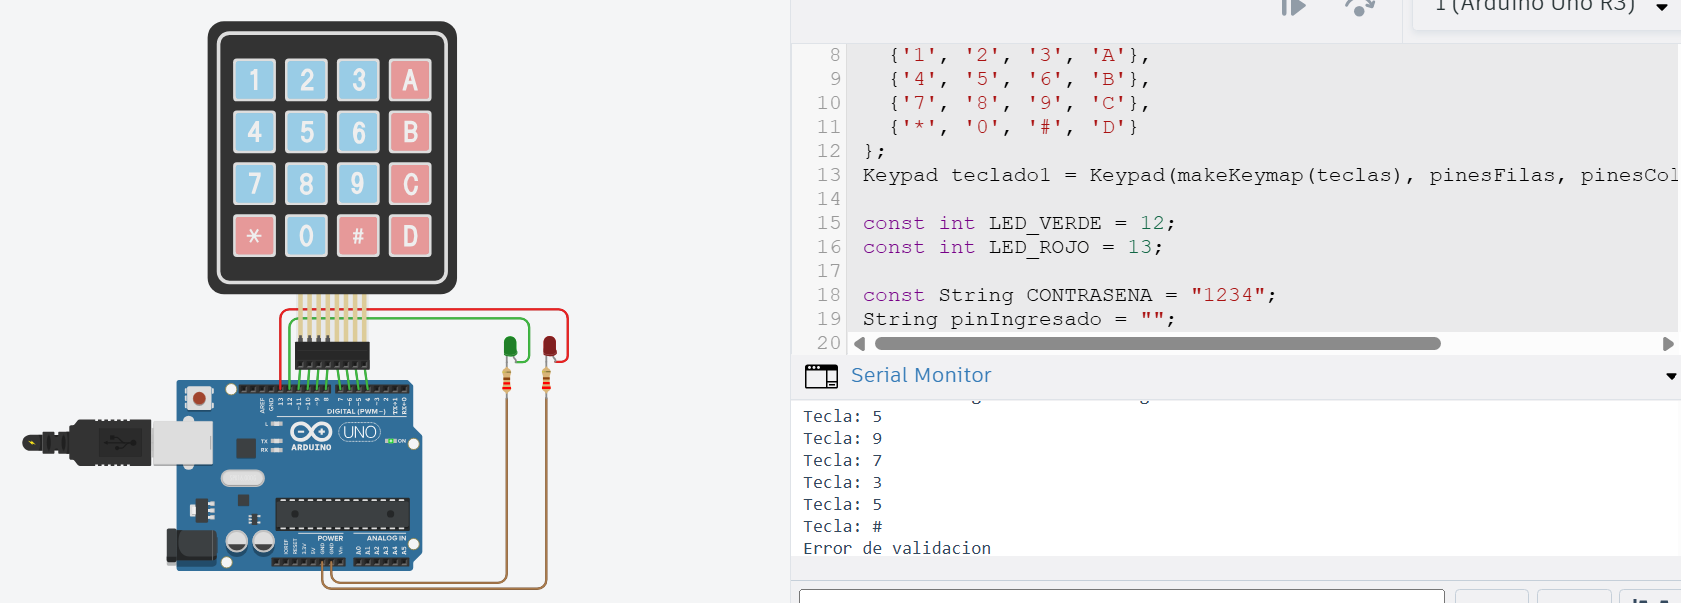
\includegraphics[width=1\linewidth]{img/14.png}
    \caption{Serial monitor incorrect pin entry.}\label{fig:14}
\end{figure}

\begin{figure}[htbp]
    \centering
    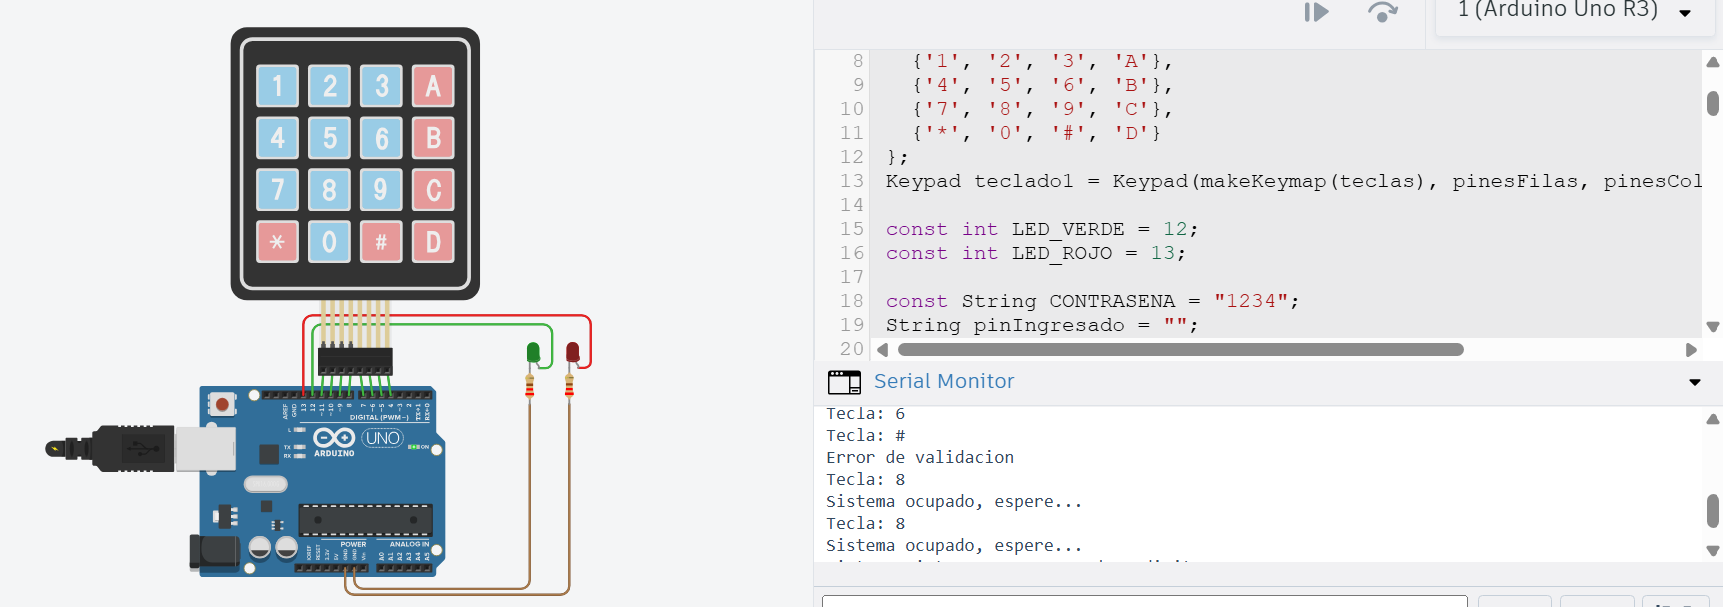
\includegraphics[width=1\linewidth]{img/15.png}
    \caption{Serial monitor busy system.}\label{fig:15}
\end{figure}

\begin{figure}[htbp]
    \centering
    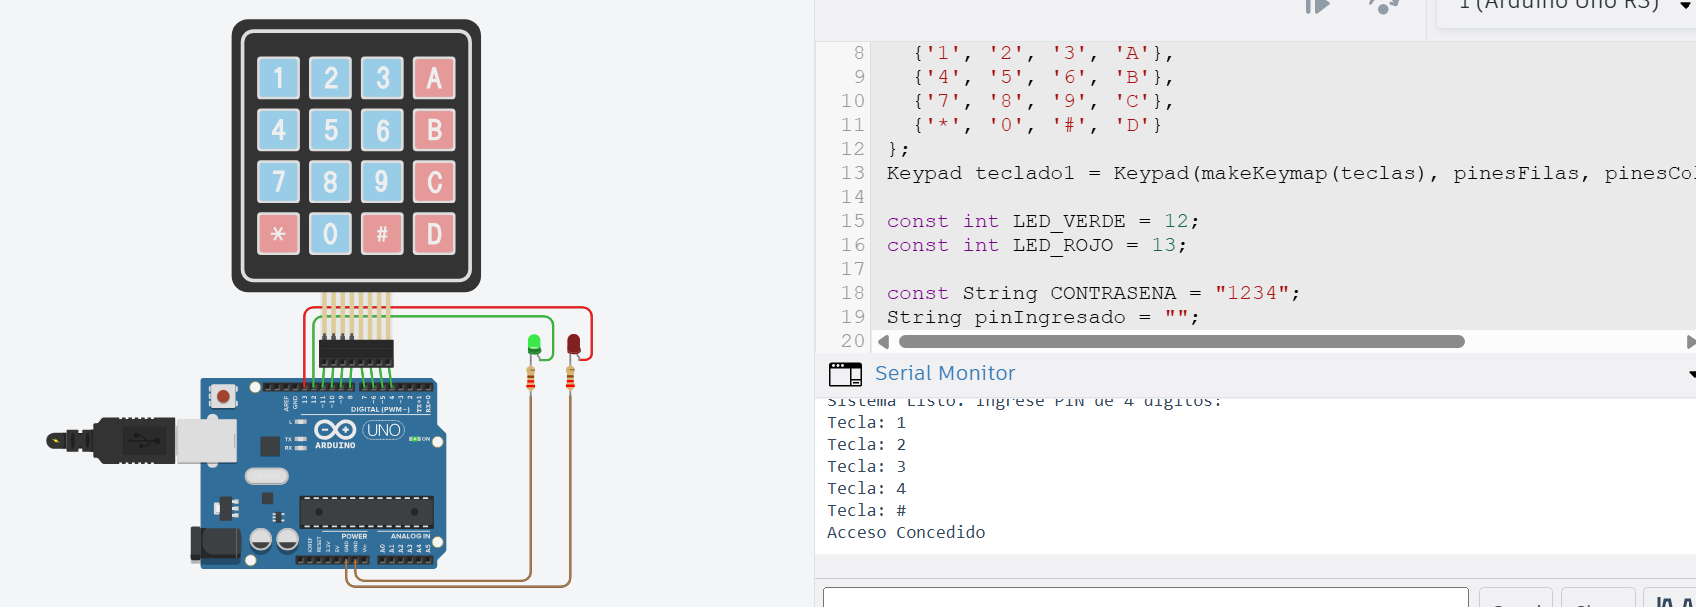
\includegraphics[width=1\linewidth]{img/16.png}
    \caption{Serial monitor successful pin entry.}\label{fig:16}
\end{figure}